% ======================================================================
% content/folien.tex  (OHNE Präambel)
% Stand: 31.01.2026 | Version: 2.5.3
% Aktualisiert: Pin-Belegung (gemeinsamer SPI), FreeRTOS-Architektur
% Farbschema: Arduino Teal + Raspberry Pi Red
% ======================================================================

% --- Folie 1: Titel (cover.pdf als Hintergrund) ------------------------
% In praesentation.tex definiert

% --- Folie 2: Hardware-Prototyp ----------------------------------------
\begin{frame}{Hardware-Prototyp v2}
\framesubtitle{10 Taster · 10 LEDs · Aufgeräumtes Layout}

\begin{columns}[c,onlytextwidth]
\column{0.48\textwidth}
\centering
\fbox{\includegraphics[width=0.95\linewidth,height=4.5cm,keepaspectratio]{images/prototyp-v2-front.png}}
\vspace{0.1cm}

{\small\textbf{Bestückungsseite} -- ESP32 + ICs}

\column{0.48\textwidth}
\centering
\fbox{\includegraphics[width=0.95\linewidth,height=4cm,keepaspectratio]{images/schaltplan.pdf}}
\vspace{0.1cm}

{\small\textbf{KiCad} -- Schaltplan}
\end{columns}

\vspace{0.2cm}
\highlight{Komponenten:} ESP32-S3 XIAO · 2× 74HC595 · 2× CD4021B · 10 LEDs · 10 Taster

\end{frame}


% --- Folie 2.5: Blockdiagramm Prototyp ---------------------------------
\begin{frame}{Schieberegister-Architektur}
\framesubtitle{Prototyp 10× -- 6 GPIO-Pins für 20 IOs}

\begin{center}
\includegraphics[width=0.85\linewidth,height=0.5\textheight,keepaspectratio]{images/prototyp-10x.png}
\end{center}

\vspace{-0.2em}

\begin{columns}[T]
\column{0.48\textwidth}
\small
\textbf{\textcolor{ArduinoTeal}{Komponenten}}
\begin{itemize}\setlength{\itemsep}{0pt}
    \item \textcolor{ArduinoTeal}{ESP32-S3 XIAO} -- Mikrocontroller
    \item \textcolor{RaspberryRed}{2× 74HC595} -- LED-Ausgabe
    \item \textcolor{SuccessGreen}{2× CD4021B} -- Taster-Eingabe
\end{itemize}

\column{0.48\textwidth}
\small
\textbf{\textcolor{ArduinoTeal}{Signale (SPI-ähnlich)}}
\begin{itemize}\setlength{\itemsep}{0pt}
    \item \textcolor{SignalData}{Data} -- SER/Q8 (grün)
    \item \textcolor{SignalClock}{Clock} -- SRCLK/CLK (gelb)
    \item \textcolor{SignalLatch}{Latch} -- RCLK/P/S (blau)
\end{itemize}
\end{columns}

\end{frame}


% --- Folie 2.7: Prototyp-Evolution -------------------------------------
\begin{frame}{Prototyp-Evolution}
\framesubtitle{v1 $\rightarrow$ v2: Von der Idee zum aufgeräumten Layout}

\begin{columns}[c,onlytextwidth]
\column{0.48\textwidth}
\centering
\fbox{\includegraphics[width=0.95\linewidth,height=2.5cm,keepaspectratio]{images/prototyp-v1-front.png}}
\vspace{0.1cm}

{\small\textbf{v1 Bestückung} -- Sockel ohne ICs}

\vspace{0.2cm}

\fbox{\includegraphics[width=0.95\linewidth,height=2.5cm,keepaspectratio]{images/prototyp-v1-back.png}}
\vspace{0.1cm}

{\small\textbf{v1 Lötseite}}

\column{0.48\textwidth}
\centering
\fbox{\includegraphics[width=0.95\linewidth,height=2.5cm,keepaspectratio]{images/prototyp-v2-front.png}}
\vspace{0.1cm}

{\small\textbf{v2 Bestückung}}

\vspace{0.2cm}

\fbox{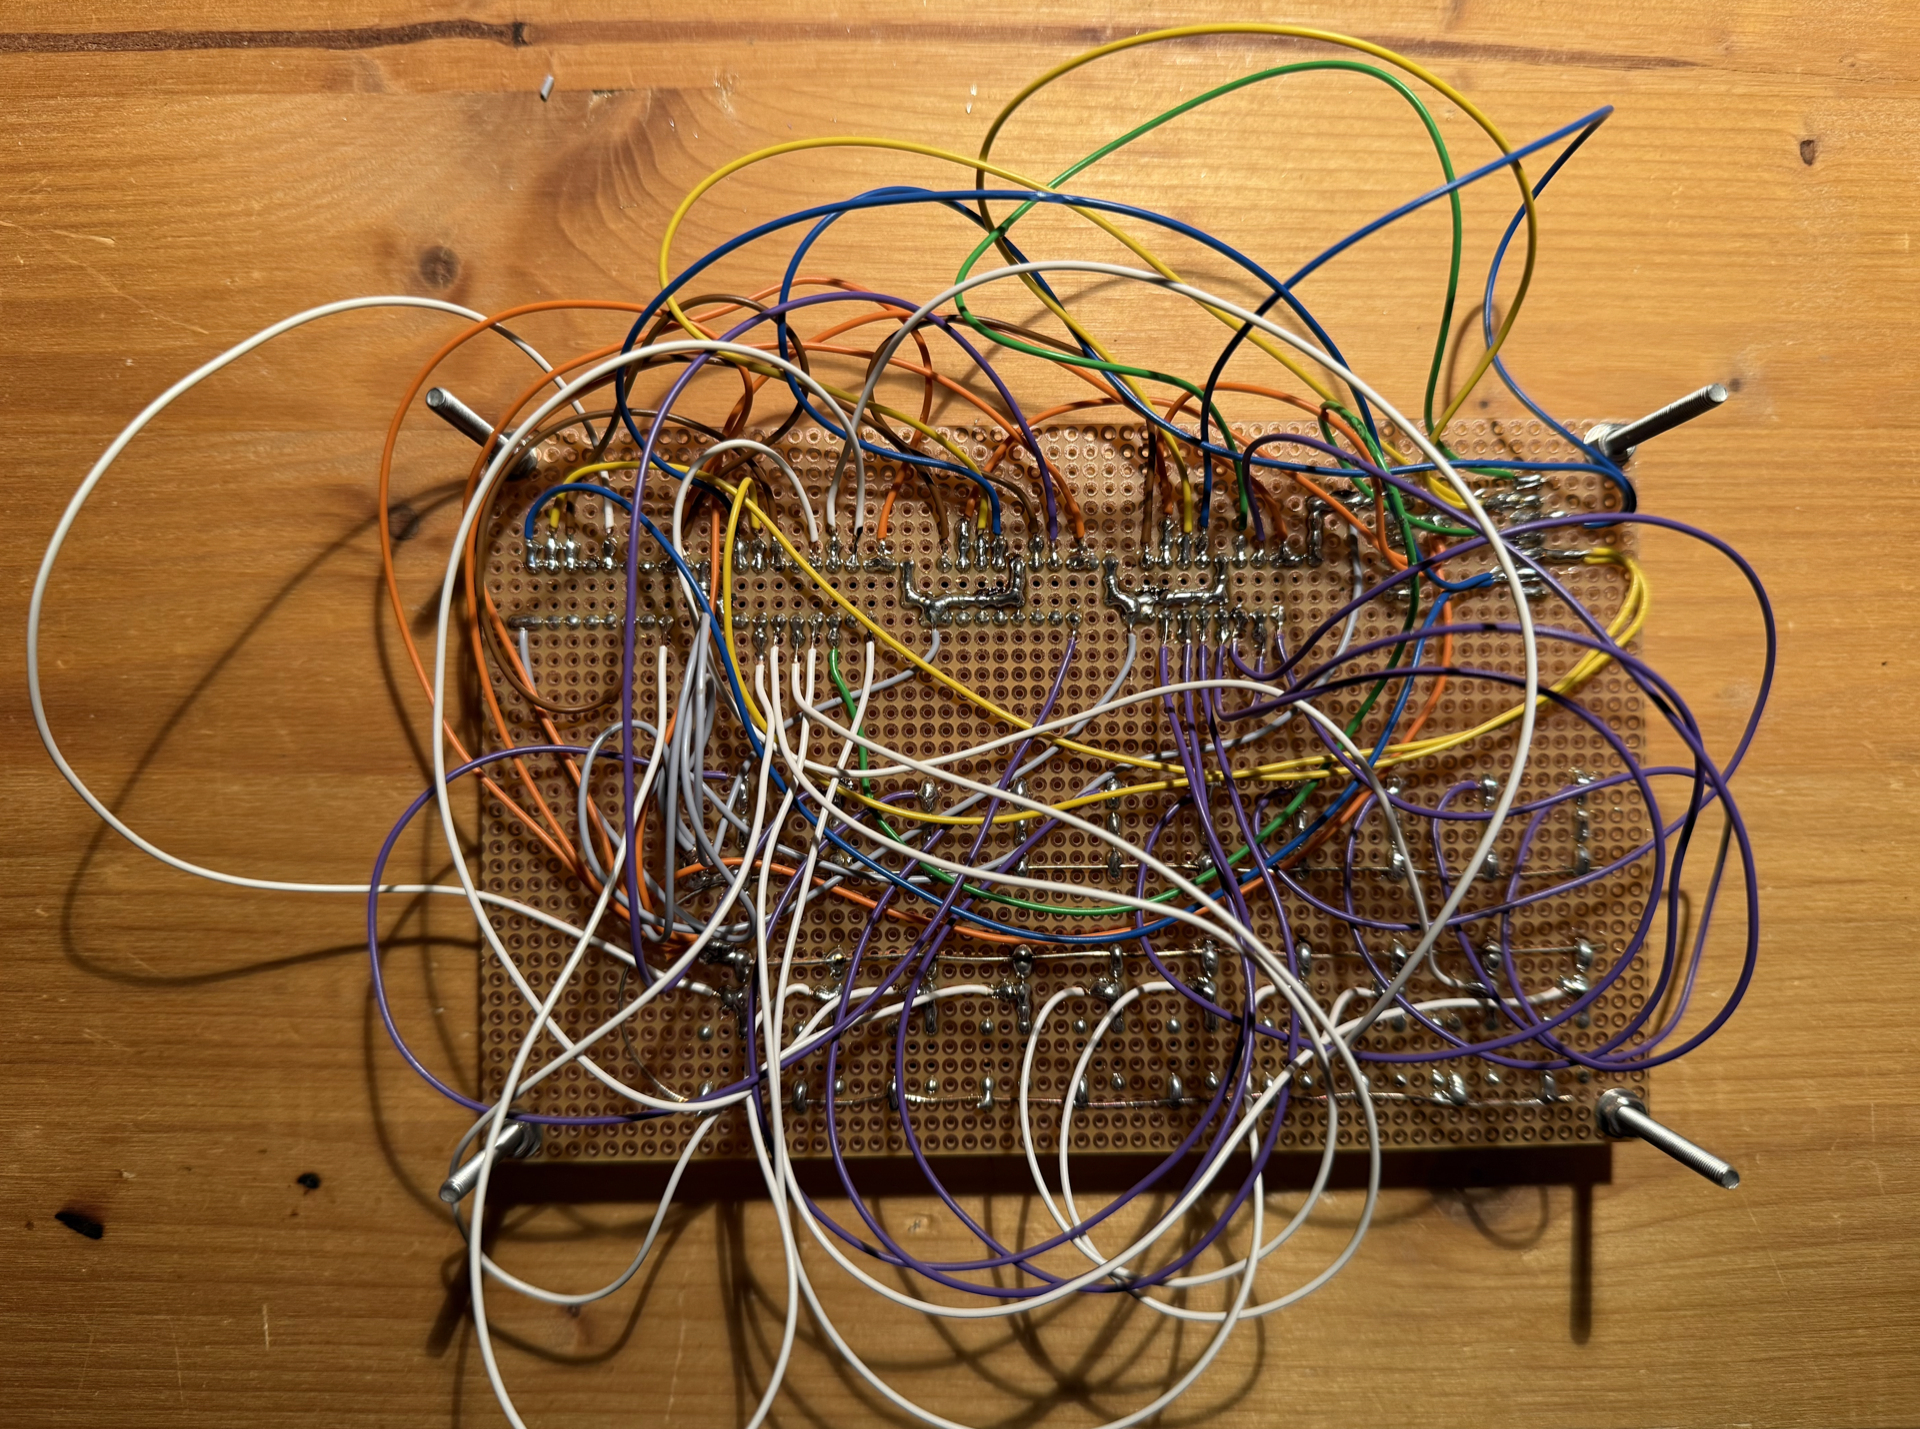
\includegraphics[width=0.95\linewidth,height=2.5cm,keepaspectratio]{images/prototyp-v2-back.png}}
\vspace{0.1cm}

{\small\textbf{v2 Lötseite}}
\end{columns}

\end{frame}


% --- Folie 3: Web-Dashboard --------------------------------------------
\begin{frame}{Web-Dashboard}
\framesubtitle{Multi-Device · Arduino/Pi Farbschema · 4K-Medien}

\begin{center}
\fbox{\includegraphics[width=0.85\linewidth,height=5cm,keepaspectratio]{images/web-dashboard4.png}}
\end{center}

\vspace{0.2cm}
\begin{columns}[T,onlytextwidth]
\column{0.24\textwidth}
\centering
\textbf{Zugriff}\\
{\small \texttt{rover:8080}}

\column{0.24\textwidth}
\centering
\textbf{Multi-Device}\\
{\small iMac, iPad, iPhone}

\column{0.24\textwidth}
\centering
\textbf{4K-Medien}\\
{\small Farbschema-Bilder}

\column{0.24\textwidth}
\centering
\textbf{Synchron}\\
{\small WebSocket Broadcast}
\end{columns}
\end{frame}


% --- Folie 4: Was ist das? ---------------------------------------------
\begin{frame}{Was ist das Auswahlpanel?}
\framesubtitle{Physische Auswahl $\rightarrow$ Digitale Reaktion}

\begin{columns}[T,onlytextwidth]
\column{0.48\textwidth}
\textbf{Anwendungsfall}
\begin{itemize}
  \item 100 physische Taster als Eingabe
  \item Jeder Taster triggert ein Bild + Audio
  \item LED zeigt aktive Auswahl an
\end{itemize}

\column{0.48\textwidth}
\textbf{Policy: \glqq{}Preempt -- Umschalten gewinnt\grqq{}}
\begin{itemize}
  \item Neuer Tastendruck $\rightarrow$ \textbf{sofortiger Wechsel}
  \item \textbf{One-hot LED:} Immer nur eine LED aktiv
  \item Nach Audio-Ende $\rightarrow$ alle LEDs aus
\end{itemize}
\end{columns}

\vspace{0.3cm}
\highlight{Merksatz:} Der letzte Tastendruck zählt -- kein Warten, kein Queue.
\end{frame}


% --- Folie 5: Systemarchitektur ----------------------------------------
\begin{frame}{Systemarchitektur -- Überblick}
\framesubtitle{Drei Ebenen: Controller · Gateway · Dashboard}

\begin{center}
\begin{tikzpicture}[
    box/.style={draw, rounded corners, minimum width=3.2cm, minimum height=1.2cm, align=center},
    arrow/.style={->, thick, >=stealth}
]
    \node[box, fill=ArduinoTeal!20] (esp) at (0,0) {\textbf{ESP32-S3}\\XIAO};
    \node[box, fill=RaspberryRed!20] (pi) at (5,0) {\textbf{Raspberry Pi 5}\\Gateway};
    \node[box, fill=SuccessGreen!20] (browser) at (10,0) {\textbf{Web-Browser}\\Dashboard};

    \draw[arrow, <->] (esp) -- node[above, font=\footnotesize] {USB-Serial} node[below, font=\footnotesize] {115200 Baud} (pi);
    \draw[arrow, <->] (pi) -- node[above, font=\footnotesize] {WebSocket} node[below, font=\footnotesize] {:8080} (browser);
\end{tikzpicture}
\end{center}

\vspace{0.3cm}
\begin{table}
\centering
\small
\begin{tabular}{@{}ll@{}}
\toprule
\textbf{Komponente} & \textbf{Aufgabe} \\
\midrule
\textcolor{ArduinoTeal}{ESP32-S3 XIAO} & 100 Taster scannen, 100 LEDs steuern, Echtzeit \\
\textcolor{RaspberryRed}{Raspberry Pi 5} & Event-Gateway, WebSocket-Server, Media-Host \\
\textcolor{SuccessGreen}{Browser} & Bild fullscreen anzeigen, Audio abspielen, Ende melden \\
\bottomrule
\end{tabular}
\end{table}
\end{frame}


% --- Folie 6: Hardware + CD4021 Timing ---------------------------------
\begin{frame}{Hardware -- Schieberegister}
\framesubtitle{100 IOs mit nur 6 GPIO-Pins}

\begin{columns}[T,onlytextwidth]
\column{0.50\textwidth}
\textbf{Warum Schieberegister?}
\begin{itemize}
  \item 100 IOs mit \textbf{6 GPIO-Pins}
  \item Kaskadierbar: $13 \times 8 = 104$ Kanäle
  \item Günstig und robust
\end{itemize}

\vspace{0.2cm}
\textbf{Pinbelegung ESP32-S3 (gemeinsamer SPI)}
\begin{table}
\footnotesize
\begin{tabular}{@{}lll@{}}
\toprule
\textbf{Signal} & \textbf{Pin} & \textbf{Funktion} \\
\midrule
SCK & D8 & SPI Clock (gemeinsam) \\
MOSI & D10 & 74HC595 SER \\
MISO & D9 & CD4021B Q8 \\
RCK & D0 & 74HC595 Latch \\
OE & D2 & 74HC595 Enable (PWM) \\
P/S & D1 & CD4021B Load \\
\bottomrule
\end{tabular}
\end{table}

\column{0.50\textwidth}
\centering
\includegraphics[width=0.98\linewidth,height=4.5cm,keepaspectratio]{images/CD4021-timing.png}

\vspace{0.1cm}
{\small\textbf{CD4021B Timing-Diagramm}}
\end{columns}

\vspace{0.1cm}
\warning{Achtung:} CD4021B hat \textbf{invertierte} Load-Logik: P/S = \textbf{HIGH} für Load!
\end{frame}


% --- Folie 7: Firmware -------------------------------------------------
\begin{frame}{Firmware -- Modulare FreeRTOS-Architektur}
\framesubtitle{Schichtentrennung: HAL · Drivers · Logic · App}

\begin{columns}[T,onlytextwidth]
\column{0.50\textwidth}
\textbf{\textcolor{ArduinoTeal}{IO-Task} (Core 1, Prio 5)}
\begin{itemize}
  \item Polling alle $5\,\mathrm{ms}$ (200\,Hz)
  \item Debouncing pro Taste ($30\,\mathrm{ms}$)
  \item Events in FreeRTOS-Queue (8 Slots)
\end{itemize}

\vspace{0.3cm}
\textbf{\textcolor{ArduinoDark}{Serial-Task} (Core 1, Prio 2)}
\begin{itemize}
  \item Log-Events aus Queue verarbeiten
  \item Debug-Ausgabe über USB-CDC
  \item Non-blocking Queue-Read
\end{itemize}

\column{0.50\textwidth}
\textbf{Schichtenmodell}
\begin{table}
\small
\begin{tabular}{@{}ll@{}}
\toprule
\textbf{Schicht} & \textbf{Inhalt} \\
\midrule
\textcolor{ArduinoTeal}{app/} & FreeRTOS Tasks \\
\textcolor{ArduinoDark}{logic/} & Debounce, Selection \\
\textcolor{RaspberryRed}{drivers/} & CD4021B, HC595 \\
\textcolor{SuccessGreen}{hal/} & SPI-Bus + Mutex \\
\bottomrule
\end{tabular}
\end{table}

\vspace{0.2cm}
\textbf{SPI-Konfiguration}
\begin{itemize}
  \item CD4021B: MODE1, 500 kHz
  \item 74HC595: MODE0, 1 MHz
  \item Mutex für Thread-Safety
\end{itemize}
\end{columns}
\end{frame}


% --- Folie 8: Protokoll ------------------------------------------------
\begin{frame}{Serial-Protokoll}
\framesubtitle{ESP32 $\leftrightarrow$ Raspberry Pi über USB-CDC (115200 Baud)}

\begin{columns}[T,onlytextwidth]
\column{0.48\textwidth}
\textbf{\textcolor{ArduinoTeal}{ESP32} $\rightarrow$ \textcolor{RaspberryRed}{Raspberry Pi}}
\begin{table}
\small
\begin{tabular}{@{}ll@{}}
\toprule
\textbf{Nachricht} & \textbf{Bedeutung} \\
\midrule
\texttt{READY} & Controller bereit \\
\texttt{FW <version>} & Firmware-Version \\
\texttt{PRESS 042} & Taster 42 gedrückt \\
\texttt{RELEASE 042} & Taster 42 losgelassen \\
\texttt{OK} & Befehl erfolgreich \\
\texttt{PONG} & Antwort auf PING \\
\bottomrule
\end{tabular}
\end{table}

\column{0.48\textwidth}
\textbf{\textcolor{RaspberryRed}{Raspberry Pi} $\rightarrow$ \textcolor{ArduinoTeal}{ESP32}}
\begin{table}
\small
\begin{tabular}{@{}ll@{}}
\toprule
\textbf{Befehl} & \textbf{Funktion} \\
\midrule
\texttt{LEDSET 042} & LED 42 ein (one-hot) \\
\texttt{LEDON/LEDOFF} & Additiv ein/aus \\
\texttt{LEDCLR/LEDALL} & Alle aus/ein \\
\texttt{PING/STATUS} & Test/Zustand \\
\texttt{TEST/STOP} & LED-Test \\
\texttt{VERSION/QRESET} & Info/Reset \\
\bottomrule
\end{tabular}
\end{table}
\end{columns}

\vspace{0.3cm}
\highlight{Debugging:} \texttt{STATUS} liefert LED-Zustand, Button-Zustand, Heap, Queue-Free, Overflow-Count.
\end{frame}


% --- Folie 9: Server ---------------------------------------------------
\begin{frame}[fragile]{Raspberry Pi Server}
\framesubtitle{Python 3.11 + aiohttp + WebSocket}

\textbf{Technologie-Stack:}
\begin{itemize}
  \item \textbf{aiohttp:} Async HTTP/WebSocket-Server
  \item \textbf{os.open + stty:} Robuste Serial-Kommunikation
  \item \textbf{Medien-Validierung:} Prüfung beim Start
  \item \textbf{systemd:} Autostart als Service
\end{itemize}

\vspace{0.3cm}
\textbf{Datenfluss bei Tastendruck:}
\begin{enumerate}
  \item \textcolor{ArduinoTeal}{ESP32} sendet \texttt{PRESS 042}
  \item \textcolor{RaspberryRed}{Server} sendet \texttt{LEDSET 042} zurück
  \item \textcolor{RaspberryRed}{Server} broadcastet \verb|{"type":"stop"}| an alle Browser
  \item \textcolor{RaspberryRed}{Server} broadcastet \verb|{"type":"play","id":42}|
  \item \textcolor{SuccessGreen}{Browser} meldet \verb|{"type":"ended","id":42}| nach Audio-Ende
  \item \textcolor{RaspberryRed}{Server} sendet \texttt{LEDCLR} (nur wenn ID noch aktuell)
\end{enumerate}

\vspace{0.2cm}
\highlight{Race-Condition-Schutz:} Ende-Event wird nur verarbeitet, wenn ID noch aktuell.
\end{frame}


% --- Folie 10: Dashboard -----------------------------------------------
\begin{frame}{Dashboard -- Implementierung}
\framesubtitle{Fullscreen-Layout · WebSocket · Audio-Unlock · Preloading}

\begin{columns}[T,onlytextwidth]
\column{0.50\textwidth}
\textbf{Features v2.5.1}
\begin{itemize}
  \item \textbf{Fullscreen:} Bild füllt Viewport
  \item \textbf{Preloading:} Alle Medien nach Unlock
  \item \textbf{WebSocket:} Auto-Reconnect (5s)
  \item \textbf{iOS-Support:} AudioContext API
\end{itemize}

\vspace{0.3cm}
\textbf{Farbschema}
\begin{itemize}
  \item \textcolor{ArduinoTeal}{Arduino Teal}: Titel, Akzente
  \item \textcolor{RaspberryRed}{Raspberry Red}: Unlock-Button
  \item \textcolor{GitHubDark}{GitHub Dark}: Hintergrund
\end{itemize}

\column{0.50\textwidth}
\textbf{Event-Handler (JavaScript)}
\begin{itemize}
  \item \texttt{stop}: Audio pausieren, \texttt{currentTime = 0}
  \item \texttt{play}: Bild + Audio aus Cache abspielen
  \item \texttt{audio.onended}: Ende-Event senden
\end{itemize}

\vspace{0.3cm}
\textbf{Medien-Mapping (1-basiert)}
\begin{itemize}
  \item ID 42 $\rightarrow$ \texttt{/media/042.jpg}
  \item ID 42 $\rightarrow$ \texttt{/media/042.mp3}
\end{itemize}
\end{columns}
\end{frame}


% --- Folie 11: Tests ---------------------------------------------------
\begin{frame}{Getestete Funktionen}
\framesubtitle{End-to-End verifiziert -- Prototyp voll funktionsfähig}

\begin{columns}[T,onlytextwidth]
\column{0.48\textwidth}
\textbf{\textcolor{ArduinoTeal}{Firmware v2.5.2 (ESP32)}}
\begin{itemize}
  \item Modulare Architektur (HAL/Drivers/Logic/App)
  \item SPI-Bus mit Mutex (Thread-safe)
  \item Debouncing: 30ms stabil
  \item Selection: One-Hot LED-Ansteuerung
  \item FreeRTOS Queue (IO $\rightarrow$ Serial)
\end{itemize}

\vspace{0.3cm}
\textbf{\textcolor{RaspberryRed}{Server v2.5.3 (Raspberry Pi)}}
\begin{itemize}
  \item Serial-Kommunikation (os.open)
  \item Robuster Parser für Fragmente
  \item WebSocket Broadcast funktioniert
\end{itemize}

\column{0.48\textwidth}
\textbf{\textcolor{SuccessGreen}{Dashboard v2.5.1 (Browser)}}
\begin{itemize}
  \item Fullscreen-Bildanzeige
  \item Audio mit Preempt-Verhalten
  \item Medien-Preloading (instant playback)
  \item Multi-Device synchron
\end{itemize}

\vspace{0.3cm}
\textbf{\textcolor{SuccessGreen}{Hardware-Prototyp}}
\begin{itemize}
  \item 10 Taster funktionsfähig
  \item 10 LEDs funktionsfähig
  \item Bit-Mapping korrekt
  \item CD4021B + 74HC595 stabil
\end{itemize}
\end{columns}
\end{frame}


% --- Folie 12: Video-Demo ----------------------------------------------
\begin{frame}{Video-Demo}
\framesubtitle{Interaktives Panel in Aktion}

\begin{center}
    \fbox{\includegraphics[width=11cm,height=4cm,keepaspectratio]{images/selection-panel.png}}

    \vspace{0.5cm}
    {\Large Video abspielen}

    \vspace{0.2cm}
    {\small\color{MutedText}Terminal: \textcolor{ArduinoTeal}{\texttt{vd}}}
\end{center}

\end{frame}


% --- Folie 13: Live-Demo -----------------------------------------------
\begin{frame}[fragile]{Live-Demo}
\framesubtitle{Hardware-Prototyp + Test-Endpoints}

\textbf{Dashboard öffnen (alle Geräte):}
\begin{verbatim}
http://rover:8080/
\end{verbatim}

\vspace{0.2cm}
\textbf{Tastendruck simulieren (ohne Hardware):}
\begin{verbatim}
curl http://rover:8080/test/play/5
\end{verbatim}

\vspace{0.2cm}
\textbf{Preempt testen (während Audio läuft):}
\begin{verbatim}
curl http://rover:8080/test/play/3
\end{verbatim}

\vspace{0.2cm}
\textbf{Status abfragen:}
\begin{verbatim}
curl http://rover:8080/status | jq
\end{verbatim}

\vspace{0.2cm}
\highlight{Hardware:} 10 Taster drücken $\rightarrow$ LED leuchtet, Bild + Audio auf allen Geräten synchron.
\end{frame}


% --- Folie 14: Ausblick + Vollausbau -----------------------------------
\begin{frame}{Ausblick: Vollausbau 100×}
\framesubtitle{Skalierung von 10 auf 100 Kanäle}

\begin{columns}[c,onlytextwidth]
\column{0.55\textwidth}
\centering
\includegraphics[width=0.98\linewidth,height=5.5cm,keepaspectratio]{images/vollausbau-100.png}

\column{0.45\textwidth}
\textbf{Änderungen für 100×}
\begin{itemize}
  \item 13× 74HC595 (statt 2×)
  \item 13× CD4021B (statt 2×)
  \item \texttt{PROTOTYPE\_MODE = false}
  \item Gleiche Firmware/Server
\end{itemize}

\vspace{0.3cm}
\textbf{Stückliste (100×)}
\begin{table}
\footnotesize
\begin{tabular}{@{}lr@{}}
\toprule
\textbf{Bauteil} & \textbf{Anzahl} \\
\midrule
74HC595 & 13× \\
CD4021B & 13× \\
LED 5mm & 100× \\
Taster & 100× \\
R 330Ω -- 3kΩ (LED) & 100× \\
R 10kΩ (Pull-up) & 100× \\
C 100nF & 26× \\
\bottomrule
\end{tabular}
\end{table}
\end{columns}

\end{frame}


% --- Folie 15: Zusammenfassung -----------------------------------------
\begin{frame}{Zusammenfassung}
\framesubtitle{Modulare Architektur, skalierbar und robust}

\begin{table}
\centering
\small
\begin{tabular}{@{}lll@{}}
\toprule
\textbf{Phase} & \textbf{Inhalt} & \textbf{Status} \\
\midrule
1 & Infrastruktur \& Toolchain & \textcolor{SuccessGreen}{$\checkmark$} \\
2 & Hardware-Prototyp (10×) & \textcolor{SuccessGreen}{$\checkmark$} \\
3 & ESP32 Firmware v2.5.2 & \textcolor{SuccessGreen}{$\checkmark$} \\
4 & Raspberry Pi Server v2.5.3 & \textcolor{SuccessGreen}{$\checkmark$} \\
5 & Web-Dashboard v2.5.1 & \textcolor{SuccessGreen}{$\checkmark$} \\
6 & Hardware-Integration (10×) & \textcolor{SuccessGreen}{$\checkmark$} \\
7 & Raspberry Pi Bridge & \textcolor{SuccessGreen}{$\checkmark$} \\
8 & 100-Button + LEDs + Multimedia & \textcolor{RaspberryRed}{$\blacktriangleleft$} Nächste Phase \\
\bottomrule
\end{tabular}
\end{table}

\vspace{0.3cm}
\highlight{Kernbotschaft:} ESP32 für Echtzeit, Pi als Gateway, Browser für UI. Skalierung 10$\rightarrow$100 per \texttt{PROTOTYPE\_MODE} Switch.

\vspace{0.2cm}
\textbf{Übertragbarkeit:} Voting-Systeme, Quiz-Panels, Museumsinstallationen.
\end{frame}


% --- Folie 16: Credits -------------------------------------------------
\begin{frame}{Credits}
\framesubtitle{Projektbeteiligte und Werkzeuge}

\begin{center}
\begin{tikzpicture}[
    box/.style={draw=ArduinoTeal, rounded corners=8pt, minimum width=10cm, minimum height=1.2cm, align=center, fill=ArduinoTeal!5},
    label/.style={font=\small\bfseries, text=ArduinoDark}
]
    % Autor
    \node[box] (autor) at (0, 2.5) {
        \textcolor{ArduinoTeal}{\Large\textbf{Jan Unger}}
    };
    \node[label, anchor=east] at (-5.5, 2.5) {Autor};

    % KI-Unterstützung
    \node[box, draw=RaspberryRed, fill=RaspberryRed!5] (ki) at (0, 0.8) {
        \textcolor{RaspberryRed}{\textbf{Claude 4.5}} · \textcolor{RaspberryRed}{\textbf{ChatGPT 5.2}}\\[0.1cm]
        {\small\color{MutedText}Text- und Code-Vorschläge}
    };
    \node[label, anchor=east] at (-5.5, 0.8) {KI-Unterstützung};

    % Hinweis
    \node[box, draw=SuccessGreen, fill=SuccessGreen!5] (hinweis) at (0, -1.0) {
        {\small\color{DarkText}Technische Prüfung und Abnahme durch den Autor}
    };
    \node[label, anchor=east] at (-5.5, -1.0) {Qualitätssicherung};
\end{tikzpicture}
\end{center}

\vspace{0.5cm}
\begin{center}
    {\color{MutedText}\rule{8cm}{0.4pt}}\\[0.3cm]
    {\small\color{MutedText}Stand: 31.01.2026}
\end{center}

\end{frame}
